\documentclass[a4paper,11pt]{exam}
\printanswers % pour imprimer les réponses (corrigé)
%\noprintanswers % Pour ne pas imprimer les réponses (énoncé)
\addpoints % Pour compter les points
% \noaddpoints % pour ne pas compter les points
%\qformat{\textbf{\thequestion ) } }
\qformat{\textbf{\thequestion )}} % Pour définir le style des questions (facultatif)
\usepackage{color} % définit une nouvelle couleur
\shadedsolutions % définit le style des réponses
% \framedsolutions % définit le style des réponses
\definecolor{SolutionColor}{rgb}{0.8,0.9,1} % bleu ciel
\renewcommand{\solutiontitle}{\noindent\textbf{Solution:}\par\noindent} % Définit le titre des solutions




\makeatletter

\def\maketitle{{\centering%
	\par{\huge\textbf{\@title}}%
	\par{\@date}%
	\par}}

\makeatother

\lhead{NOM Pr\'enom :}
\rhead{\textbf{Les r\'eponses doivent \^etre justifi\'ees}}
\cfoot{\thepage / \pageref{LastPage}}


%\usepackage{../../pas-math}
%\usepackage{../../moncours}


%\usepackage{pas-cours}
%-------------------------------------------------------------------------------
%          -Packages nécessaires pour écrire en Français et en UTF8-
%-------------------------------------------------------------------------------
\usepackage[utf8]{inputenc}
\usepackage[frenchb]{babel}
\usepackage[T1]{fontenc}
\usepackage{lmodern}
\usepackage{textcomp}



%-------------------------------------------------------------------------------

%-------------------------------------------------------------------------------
%                          -Outils de mise en forme-
%-------------------------------------------------------------------------------
\usepackage{hyperref}
\hypersetup{pdfstartview=XYZ}
%\usepackage{enumerate}
\usepackage{graphicx}
\usepackage{multicol}
\usepackage{tabularx}
\usepackage{multirow}


\usepackage{anysize} %%pour pouvoir mettre les marges qu'on veut
%\marginsize{2.5cm}{2.5cm}{2.5cm}{2.5cm}

\usepackage{indentfirst} %%pour que les premier paragraphes soient aussi indentés
\usepackage{verbatim}
\usepackage{enumitem}
\usepackage[usenames,dvipsnames,svgnames,table]{xcolor}

\usepackage{variations}

%-------------------------------------------------------------------------------


%-------------------------------------------------------------------------------
%                  -Nécessaires pour écrire des mathématiques-
%-------------------------------------------------------------------------------
\usepackage{amsfonts}
\usepackage{amssymb}
\usepackage{amsmath}
\usepackage{amsthm}
\usepackage{tikz}
\usepackage{xlop}
%-------------------------------------------------------------------------------



%-------------------------------------------------------------------------------


%-------------------------------------------------------------------------------
%                    - Mise en forme avancée
%-------------------------------------------------------------------------------

\usepackage{ifthen}
\usepackage{ifmtarg}


\newcommand{\ifTrue}[2]{\ifthenelse{\equal{#1}{true}}{#2}{$\qquad \qquad$}}

%-------------------------------------------------------------------------------

%-------------------------------------------------------------------------------
%                     -Mise en forme d'exercices-
%-------------------------------------------------------------------------------
%\newtheoremstyle{exostyle}
%{\topsep}% espace avant
%{\topsep}% espace apres
%{}% Police utilisee par le style de thm
%{}% Indentation (vide = aucune, \parindent = indentation paragraphe)
%{\bfseries}% Police du titre de thm
%{.}% Signe de ponctuation apres le titre du thm
%{ }% Espace apres le titre du thm (\newline = linebreak)
%{\thmname{#1}\thmnumber{ #2}\thmnote{. \normalfont{\textit{#3}}}}% composants du titre du thm : \thmname = nom du thm, \thmnumber = numéro du thm, \thmnote = sous-titre du thm

%\theoremstyle{exostyle}
%\newtheorem{exercice}{Exercice}
%
%\newenvironment{questions}{
%\begin{enumerate}[\hspace{12pt}\bfseries\itshape a.]}{\end{enumerate}
%} %mettre un 1 à la place du a si on veut des numéros au lieu de lettres pour les questions 
%-------------------------------------------------------------------------------

%-------------------------------------------------------------------------------
%                    - Mise en forme de tableaux -
%-------------------------------------------------------------------------------

\renewcommand{\arraystretch}{1.7}

\setlength{\tabcolsep}{1.2cm}

%-------------------------------------------------------------------------------



%-------------------------------------------------------------------------------
%                    - Racourcis d'écriture -
%-------------------------------------------------------------------------------

% Angles orientés (couples de vecteurs)
\newcommand{\aopp}[2]{(\vec{#1}, \vec{#2})} %Les deuc vecteurs sont positifs
\newcommand{\aopn}[2]{(\vec{#1}, -\vec{#2})} %Le second vecteur est négatif
\newcommand{\aonp}[2]{(-\vec{#1}, \vec{#2})} %Le premier vecteur est négatif
\newcommand{\aonn}[2]{(-\vec{#1}, -\vec{#2})} %Les deux vecteurs sont négatifs

%Ensembles mathématiques
\newcommand{\naturels}{\mathbb{N}} %Nombres naturels
\newcommand{\relatifs}{\mathbb{Z}} %Nombres relatifs
\newcommand{\rationnels}{\mathbb{Q}} %Nombres rationnels
\newcommand{\reels}{\mathbb{R}} %Nombres réels
\newcommand{\complexes}{\mathbb{C}} %Nombres complexes


%Intégration des parenthèses aux cosinus
\newcommand{\cosP}[1]{\cos\left(#1\right)}
\newcommand{\sinP}[1]{\sin\left(#1\right)}


%Probas stats
\newcommand{\stat}{statistique}
\newcommand{\stats}{statistiques}
%-------------------------------------------------------------------------------

%-------------------------------------------------------------------------------
%                    - Mise en page -
%-------------------------------------------------------------------------------

\newcommand{\twoCol}[1]{\begin{multicols}{2}#1\end{multicols}}


\setenumerate[1]{font=\bfseries,label=\textit{\alph*})}
\setenumerate[2]{font=\bfseries,label=\arabic*)}


%-------------------------------------------------------------------------------
%                    - Elements cours -
%-------------------------------------------------------------------------------





%\usepackage{fullpage}
\author{\ }
\date{18 Octobre 2017}
\title{Terminale ST$_2$S : DS num\'ero 1}


\begin{document}
%	\usepackage{fancyhdr}
%	
%	\pagestyle{fancy}
%	\fancyhf{}
	%\rhead{Share\LaTeX}

	\maketitle

\section{Effectifs étudiants}
	
	\begin{questions}
		\question En 2005, \num{125634} étudiants se sont inscrits en IUT. Environ \num{33.8}\% venaient de série technologiques. Combien d'élèves inscrits en IUT en 2005 venaient de séries technologiques ?
		\begin{solution}
			$ \num{125634} \times \dfrac{\num{33.8}}{100} = \num{42464.292} $ \\
			Soit environ \num{42465} étudiants issus de séries technologiques.
		\end{solution}
		
		\question Au lycée Marcel PAGNOL, 62 élèves sont inscrits en section ST2S, ce qui représente 8\% du total des élèves. Combien y a t-il d'élèves dans ce lycée ?
		\begin{solution}
			$ \dfrac{\num{62}}{\num{0.08}} = 775 $ \\
			Soit environ 775 élèves dans le lycée.
		\end{solution}
	\end{questions}


\section{Efficacité d'un médicament}

120 personnes atteintes d'une maladie ont accepté de tester l'efficacité d'un nouveau médicament. 

Pendant un mois 80 personnes parmi elles ont pris le médicament, les autres ont prit le placebo.

A l'issue de l'expérimentation :
\begin{itemize}
	\item parmi les personnes ayant pris le médicament, 75\% ont vu leur santé s'améliorer;
	\item parmi les personnes ayant prit le placebo, seulement 5 personnes ont vu leur santé s'améliorer.
\end{itemize} 
\begin{center}
	
{\small \begin{tabular}{|@{\ }c@{\ }|@{\ }c@{\ }|@{\ }c@{\ }|@{\ }c@{\ }|}
	\hline
	& Ont vu leur santé s'améliorer & N'ont pas vu leur santé s'améliorer &  Total  \\
	\hline
	Ont pris le médicament &  &  &    \\
	\hline
	Ont prit le placebo &  &  &   \\
	\hline
	Total &  &  & 120   \\
	\hline
\end{tabular}}
\end{center}


\begin{questions}
	\question Compléter le tableau.
	
	\begin{solution}
		{\small \begin{tabular}{|@{\ }c@{\ }|@{\ }c@{\ }|@{\ }c@{\ }|@{\ }c@{\ }|}
				\hline
				& Ont vu leur santé s'améliorer & N'ont pas vu leur santé s'améliorer &  Total  \\
				\hline
				Ont pris le médicament &  60 & 20 & 80   \\
				\hline
				Ont prit le placebo & 5 & 35 &  40 \\
				\hline
				Total &  65 & 55 & 120   \\
				\hline
		\end{tabular}}
	
	\end{solution}
	\question \begin{parts}
		\part Calculer le pourcentage de personnes qui ont vu leu santé s'améliorer (arrondir à \num{0.01}\% près).
		\begin{solution}
			$ \dfrac{65}{120} \approx \num{0.5417} $ Soit \num{54.17} \%.
		\end{solution}
		\part Parmi les personnes qui n'ont pas prit le médicament, calculer le pourcentage de celles qui ont vu leur santé s'améliorer.
		\begin{solution}
			$ \dfrac{60}{80} = \num{0.75} $ Soit \num{75} \%.
		\end{solution}
		\part Parmi les personnes qui ont vu leur santé s'améliorer, calculer le pourcentage de celles qui ont prit le médicament (arrondir à \num{0.1}\% près).
		\begin{solution}
			$ \dfrac{60}{65} \approx \num{0.923} $ Soit \num{92.3} \%.
		\end{solution}
	\end{parts}
\end{questions}

%\section{A propos des acides gras oméga-3}
%On a récemment découvert que les acides gras oméga-3, présents dans des poissons comme la truite ou le saumon, ont un effet protecteur contre les maladies cardio-vasculaires.
%\emph{Les pourcentages demandés seront arrondis à \num{e-2}. \%} 
%
%\begin{questions}
%	\question Une portion de 180 g de saumon d'élevage fournit environ \num{1.5}g d'oméga-3. Calculer le pourcentage d'oméga-3 dans le saumon d'élevage.
%	\begin{solution}
%		$\dfrac{\num{1.5}}{\num{180}} \approx \num{0.0083}$, soit \num{0.83} \% d'oméga-3 dans le saumon d'élevage.
%	\end{solution}
%	
%	\question Le pourcentage d'omega-3 dans le saumon sauvage est de \num{0.78} \%. En déduire la quantité d'oméga-3 contenue dans une portion de 180g de saumon sauvage (arrondir à \num{0.1} g).
%	\begin{solution}
%		$180 \times \frac{\num{0.78}}{100} = \num{1.404}$, soit environ \num{1.4} g d'oméga-3 pour 180 g de saumon sauvage.
%	\end{solution}
%	
%	\question Consigner les résultats précédents dans le tableau suivant et finir de le compléter. Le détail des calculs n'est pas demandé.
%	
%	{\footnotesize \begin{tabular}{@{\ }c@{\ }|@{\ }c@{\ }|@{\ }c@{\ }|@{\ }c@{\ }|@{\ }c@{\ }|}
%		\cline{2-5}
%		& \multicolumn{2}{c|}{Elevage}               & \multicolumn{2}{c|}{Sauvage}               \\ \cline{2-5} 
%		& Pourcentage d'oméga-3 & Quantité d'oméga-3 & Pourcentage d'oméga-3 & Quantité d'oméga-3 \\ \hline
%		\multicolumn{1}{|@{\ }c@{\ }|}{Saumon (180 g)} &                       & \num{1.5} g      & \num{0.78}\%        &                    \\ \hline
%		\multicolumn{1}{|@{\ }c@{\ }|}{Truite (180 g)} &                       & \num{1.3} g      & \num{0.22}\%        &                    \\ \hline
%	\end{tabular}}
%	
%	\begin{solution}
%		{\footnotesize \begin{tabular}{@{\ }c@{\ }|@{\ }c@{\ }|@{\ }c@{\ }|@{\ }c@{\ }|@{\ }c@{\ }|}
%				\cline{2-5}
%				& \multicolumn{2}{c|}{Elevage}               & \multicolumn{2}{c|}{Sauvage}               \\ \cline{2-5} 
%				& Pourcentage d'oméga-3 & Quantité d'oméga-3 & Pourcentage d'oméga-3 & Quantité d'oméga-3 \\ \hline
%				\multicolumn{1}{|@{\ }c@{\ }|}{Saumon (180 g)} &  \num{0.83} \%   & \num{1.5} g      & \num{0.78}\%        &    \num{1.4} g                \\ \hline
%				\multicolumn{1}{|@{\ }c@{\ }|}{Truite (180 g)} &  \num{0.72} \%  & \num{1.3} g      & \num{0.22}\%        &  \num{0.4} g\\ \hline
%			\end{tabular}}
%	\end{solution}
%	
%	\question La consommation d'une portion de 180 g de truite d'élevage couvre environ 37 \% des besoins hebdomadaires d'un être humain. Montrer que ces besoins, arrondis à \num{0.1} g, sont de \num{3.5} g.
%	
%	\begin{solution}
%		Soit $x$ le besoin hebdomadaire en oméga-3 d'un être humain. On a $\dfrac{37 \times x}{100}=\num{1.3}$.
%		
%		Donc $x=\dfrac{\num{1.3}}{\num{0.37}} \approx \num{3.51}$ g.
%	\end{solution} 
%	
%	\question Retrouver la réponse précédente sachant que ces besoins hebdomadaires sont exactement couverts si on consomme 450 g de saumon sauvage.
%	\begin{solution}
%		$\dfrac{450 \times \num{0.78}}{100} = \num{3.51}$ soit \num{3.5} g.
%	\end{solution}
%	
%	\question Calculer la quantité de truite sauvage qu'il faudrait consommer pour couvrir la totalité de ces besoins hebdomadaires (arrondir à 10 g).
%	\begin{solution}
%		$\dfrac{\num{3.5}}{\num{0.4}}\times 180 = 1575$, soit 1570 g de truite sauvage pour couvrir les besoins hebdomadaires en oméga-3. 
%	\end{solution}
%\end{questions}


\newpage

\section{\'Evolution de la population de deux communes}
	
	
	Le graphique ci-dessous représente l'évolution du nombre d'habitants de deux communes voisines, nommées A et B, de l'année 1986 à l'année 2010 (de quatre années en quatre années) .
	
	\begin{center}
		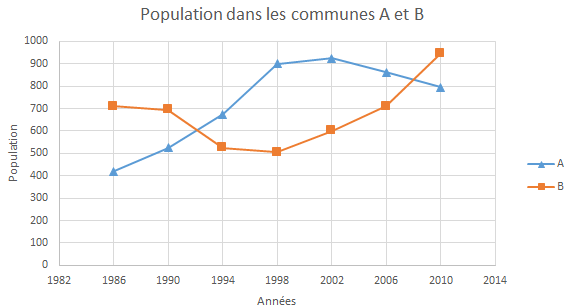
\includegraphics[scale=0.7]{./graph}
	\end{center}


\subsection{Lecture graphique}				

Répondre aux questions suivantes en utilisant uniquement le graphique ci-dessus.

\begin{questions}
	\question En quelle année, la population de la commune A a été maximale ?
	\begin{solution}
		La population de la commune A a été maximale en 2002.
	\end{solution}
	
	\question Préciser les années où les deux communes on eu le même nombre d'habitants.
	\begin{solution}
		Les deux villes ont eu la même population en 1992 et 2008.
	\end{solution}
	
	\question Quelles sont les périodes où la commune B a eu plus d'habitants que la commune A.
	\begin{solution}
		La commune B a eu plus d'habitants que la commune A entre 1986 et 1992 et entre 2008 et 2010.
	\end{solution}
	
	\question En quelle année l'écart entre le nombre d'habitants des deux communes a-t-il été le plus important.
	\begin{solution}
		L'écart entre les deux communes a été le plus important en 1998.
	\end{solution}
	
	\question Préciser, en justifiant la réponse, pendant quelle période de quatre années, la commune A a eu la plus forte augmentation de sa population.
	\begin{solution}
		La plus forte augmentation de la population de la commune A a eu lieu entre 1994 et 1998. L'angle de la pente de la courbe est la plus importante sur cette période.
	\end{solution}
\end{questions}

\subsection{Pourcentage d'évolution}

\begin{multicols}{2}

\vspace*{0.1cm}	
On s'intéresse à l'évolution de la population dans ces communes entre 2006 et 2010. Le tableau suivant indique le nombre d'habitants dans ces deux communes en 2006 et en 2010. 



	\begin{tabular}{|@{\ }c@{\ }|@{\ }c@{\ }|@{\ }c@{\ }|}
		\hline
		\textbf{Années} & \textbf{2006} & \textbf{2010}\\
		\hline
		\textbf{Commune A} & \num{863} & \num{795}  \\
		\hline 
		\textbf{Commune B} & \num{711} & \num{947}  \\
		\hline
	\end{tabular}

\end{multicols}	

Les questions sont indépendantes.

\begin{questions}
	\question Justifier que, de 2006 à 2010, la population à baissé d'environ \num{7.9} \%.
	\begin{solution}
		$\dfrac{795 - 863}{863} \approx \num{-0.079} $, soit une baisse de \num{7.9} \%.
	\end{solution}
	
	\question Déterminer le pourcentage d'augmentation de la population de la commune B dans cette même période (on donnera le résultat arrondi à \num{0.1} \%).
	\begin{solution}
		$\dfrac{947-711}{711}\approx \num{0.331}$, soit une hausse de \num{33.1}\%.
	\end{solution}
	
	\question Si on considère la population des deux communes réunies, déterminer le pourcentage de cette évolution pendant durant cette période (on donnera le résultat arrondi à \num{0.1} \%).
	\begin{solution}
		\begin{itemize}
			\item Population globale en 2006 : $863 + 711 = 1574$ habitants.
			\item Population globale en 2010 : $795 + 947 = 1742$ habitants.
			\item \'Evolution globale : $\dfrac{1742-1574}{1574} \approx \num{0.107}$, soit une hausse de \num{10.7} \%.
		\end{itemize}
	\end{solution}
	
\end{questions}


\section{Le laboratoire perd du terrain}

Le chiffre d'affaires annuel d'un laboratoire pharmaceutique était en 2008 de \num{32860000} euros et en 2009 de \num{28947000} euros.
\begin{questions}
	\question Calculer le pourcentage de baisse du chiffre d'affaire de l'entreprise entre 2008 et 2009. Arrondir à \num{0.01} \%.
	\begin{solution}
		$\dfrac{\num{28947000} - \num{32860000}}{\num{32860000}} \approx \num{-0.1191}$, soit une baisse de \num{11.91} \%.
	\end{solution}
	
	\question Calculer le pourcentage de hausse qui ramènerait, en 2010, le chiffre d'affaires au niveau de 2008. Arrondir les coefficients multiplicateurs à \num{e-4}.
	\begin{solution}
		Le coefficient multiplicateur correspondant à une baisse de \num{11.91} \% est ($1-\num{0.1191} = \num{0.8809}$).
		
		$\dfrac{1}{\num{0.8809}} = \num{1.1352}$, soit une hausse de \num{13.52} \%.
	\end{solution}
\end{questions}


\section{Personnel hospitalier}

Dans un hôpital; 30\% du personnel est composé de médecins et 50\% est composé d'infirmiers. Peut-on en conclure que dans cet hôpital, le nombre de médecins est inférieur au nombre d'infirmiers ? Justifier la réponse.

\begin{solution}
	La proportion de médecins et d'infirmiers se rapportent à la même population (le personnel de l'hôpital). 30 est inférieur à 50, donc il y a moins de médecins que d'infirmiers.
\end{solution}

	\label{LastPage}
	

\end{document}